

\tikzset{every picture/.style={line width=0.75pt}} %set default line width to 0.75pt

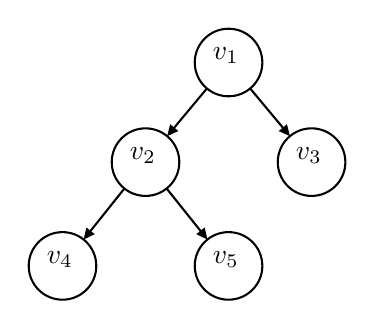
\begin{tikzpicture}[x=0.75pt,y=0.75pt,yscale=-1,xscale=1]
%uncomment if require: \path (0,151); %set diagram left start at 0, and has height of 151


% Text Node
\draw    (110, 21) circle [x radius= 16.28, y radius= 16.28]   ;
\draw (101,12.4) node [anchor=north west][inner sep=0.75pt]    {$v_{1}$};
% Text Node
\draw    (70, 69) circle [x radius= 16.28, y radius= 16.28]   ;
\draw (61,60.4) node [anchor=north west][inner sep=0.75pt]    {$v_{2}$};
% Text Node
\draw    (30, 119) circle [x radius= 16.28, y radius= 16.28]   ;
\draw (21,110.4) node [anchor=north west][inner sep=0.75pt]    {$v_{4}$};
% Text Node
\draw    (150, 69) circle [x radius= 16.28, y radius= 16.28]   ;
\draw (141,60.4) node [anchor=north west][inner sep=0.75pt]    {$v_{3}$};
% Text Node
\draw    (110, 119) circle [x radius= 16.28, y radius= 16.28]   ;
\draw (101,110.4) node [anchor=north west][inner sep=0.75pt]    {$v_{5}$};
% Connection
\draw    (99.58,33.51) -- (82.34,54.19) ;
\draw [shift={(80.42,56.49)}, rotate = 309.81] [fill={rgb, 255:red, 0; green, 0; blue, 0 }  ][line width=0.08]  [draw opacity=0] (5.36,-2.57) -- (0,0) -- (5.36,2.57) -- cycle    ;
% Connection
\draw    (59.83,81.71) -- (42.04,103.95) ;
\draw [shift={(40.17,106.29)}, rotate = 308.65999999999997] [fill={rgb, 255:red, 0; green, 0; blue, 0 }  ][line width=0.08]  [draw opacity=0] (5.36,-2.57) -- (0,0) -- (5.36,2.57) -- cycle    ;
% Connection
\draw    (80.17,81.71) -- (97.96,103.95) ;
\draw [shift={(99.83,106.29)}, rotate = 231.34] [fill={rgb, 255:red, 0; green, 0; blue, 0 }  ][line width=0.08]  [draw opacity=0] (5.36,-2.57) -- (0,0) -- (5.36,2.57) -- cycle    ;
% Connection
\draw    (120.42,33.51) -- (137.66,54.19) ;
\draw [shift={(139.58,56.49)}, rotate = 230.19] [fill={rgb, 255:red, 0; green, 0; blue, 0 }  ][line width=0.08]  [draw opacity=0] (5.36,-2.57) -- (0,0) -- (5.36,2.57) -- cycle    ;

\end{tikzpicture}